\documentclass[11pt]{ctexart}

\usepackage[S]{dryNote}
\usepackage{dryNotation}
\usepackage{tabularx}
\usepackage[toc]{multitoc}
\usepackage{gbt7714}
\usepackage{longtable}

\title{概率论与数理统计习题课-2\textsuperscript{nd}}
\author{例题讲解}
\date{2024年11月16日}

\begin{document}
\maketitle
{ 	
	\footnotesize
	\keben
	\tableofcontents
}

\addtocontents{toc}{\protect\setcounter{tocdepth}{2}}

%%%%%%%%%%%%%%%%%%%%%%%%%%%%%%%%%%%%%%%%%%%%%%%%%%%%%%%%%%%%%%%%%%%%%%%%



\section{常用分布及其数字特征}

\subsection{基础知识}

随机变量$X$的\textbf{数学期望}为$E(X)$, 它的\text{方差}为$D(X) = E[(X - E(X))^2] = E(X^2) - [E(X)]^2 \geq 0$, 标准差为$\sqrt{D(X)}$. 
特别地, 当$X$为\textbf{离散型}随机变量时, 
\begin{equation*}
	E(X) = \sum_{k=1}^{\infty} x_k p_k, \quad E(X^2) = \sum_{k=1}^{\infty} x_k^2 p_k. 
\end{equation*}
当$X$为\textbf{连续型}随机变量时, 
\begin{equation*}
	E(X) = \int_{-\infty}^{+\infty} x f(x) \dd x, \quad E(X^2) = \int_{-\infty}^{+\infty} x^2 f(x) \dd x. 
\end{equation*}

由定义不难得出, 期望具有线性性质
\begin{equation*}
	E(aX + b) = aE(X) + b, 
\end{equation*}
而方差则不然
\begin{equation*}
	D(aX+ b) = a^2 D(X).
\end{equation*}
此外期望具有可加性$E(X+Y) = E(X) + E(Y)$. 


\begin{table}[H]
	\centering
	\begin{tabular}{c|c|c|c}
	\toprule
		分布 & 分布律$p_k$或概率密度$f(x)$ & 期望 & 方差 \\
	\midrule
		二项分布 $B(n,p)$ & $p_k = C_n^k p^k (1-p)^{n-k}$ & $np$ & $np(1-p)$ \\
	\midrule
		泊松分布 $\pi(\lambda)$ & $p_k = \frac{\lambda^k e^{-\lambda}}{k !}$ & $\lambda$ & $\lambda$ \\
	\midrule
		均匀分布 $U(a, b)$ & $f(x) = \begin{cases} \frac{1}{b-a} & x \in (a, b) \\ 0, &\textbf{其它} \end{cases}$ & $\frac{a+b}2$ & $\frac{(b-a)^2}{12}$  \\
	\midrule 
		正态分布 $N(\mu,\sigma^2)$ & $f(x) = \frac{1}{\sqrt{2 \pi} \sigma} e^{- \frac{(x-\mu)^2}{2 \sigma^2}}$ & $\mu$ & $\sigma^2$ \\
	\midrule 
		指数分布 $Exp(\lambda)$ & $f(x) = \begin{cases}\lambda e^{-\lambda x}, & x > 0, \\
			0, & x\leq 0, \end{cases}$ & $\frac{1}{\lambda}$ & $\frac{1}{\lambda^2}$ \\
	\bottomrule
	\end{tabular}
	\caption{常用分布的数学期望和方差}
\end{table}

\textbf{切比雪夫不等式}给出了随机变量$X$和其数学期望之间偏差的粗糙估计: 若随机变量$X$的期望和方差均存在, 那么对任意$\varepsilon > 0$, 都有
\begin{equation*}
	P\{|X - E(X)| \geq \varepsilon\} \leq \frac{D(X)}{\varepsilon^2}. 
\end{equation*}
\begin{proof}
	当$X$为连续型随机变量时, 
	\begin{align*}
		& P\{|X - E(X)| \geq \varepsilon\} \\
		= & \int_{\{x \colon |x - E(X)| \geq \varepsilon\}} p(x) \dd x
		\leq  \int_{\{x \colon |x - E(X)| \geq \varepsilon\}} \frac{(x-E(X))^2}{\varepsilon^2} p(x) \dd x \\
		\leq & \frac{1}{\varepsilon^2} \int_{-\infty}^{+\infty} (x-E(X))^2 p(x) \dd x
		= \frac{D(X)}{\varepsilon^2}. 
	\end{align*}
\end{proof}

\subsection{例题示范}

\begin{example}
	一直$E(X)=-2$,$E(X^{2})=5$, 求 $D(1-3X)$.
\end{example}
\begin{solution}
	$D(1-3X)=9D(X)=9[\:E(X^{2})\:-\:(\:E(X)\:)^{2}\:]=9[\:5-4\:]=9$.
\end{solution}

\begin{example}
	设随机变量 $X\sim B(n,p)$,已知$E(X)=2.4$, $D(X)=1.44$, 求两个参数$n$与$p$. 
\end{example}
\begin{solution}
	由$np = E(X) = 2.4$, $np(1-p) = D(X) = 1.44$可知$n=6, p = 0.4$. 
\end{solution}

\begin{example}
	若随机变量$X \sim N(\mu, \sigma^2)$, 方程$x^2 + 4x + K = 0$无实根的概率为$0.5$, 求$\mu$. 
\end{example}
\begin{solution}
	方程无实根等价于$16 - 4K < 0$, 于是
	\begin{equation*}
		0.5 
		= P\{K > 4\} 
		= 1 - P\left(\frac{K - \mu}{\sigma} \leq \frac{4 - \mu}{\sigma} \right)
		= 1 - \Phi\left(\frac{4 - \mu}{\sigma} \right), 
	\end{equation*}
	由此知$\mu = 4$. 
\end{solution}
\begin{example}
	某种圆盘的直径在区间$(a,b)$上服从均匀分布,试求此种圆盘的平均面积. 
\end{example}
\begin{solution}
	记$X$为圆盘的直径,则圆盘的面积为$Y=\pi X^2/4$,所以平均面积为
	\begin{equation*}
		E(Y) 
		= \frac{\pi}{4} E(X^2) 
		= \frac{\pi}{4} \int_a^b \frac{x^2}{b-a} \dd x
		= \frac{\pi}{12} (a^2 + ab + b^2). 
	\end{equation*}
\end{solution}
\begin{example}
	若一次电话通话时间$X$(以min计)服从参数为$0.25$的指数分布,试求一次通话的平均时间. 
\end{example}
\begin{solution}
	由$X \sim Exp(\lambda)$, $E(X) = \frac{1}{\lambda} = 4$(min). 
\end{solution}
\begin{example}
	写出以下正态分布的均值和标准差:
	\begin{equation*}
		f_{1}\left(x\right)=\frac{1}{\sqrt{\pi}}\mathrm{e}^{-\left(x^2+4x+4\right)}, \quad
		f_{2}\left(x\right)=\sqrt{\frac{2}{\pi}}\mathrm{e}^{-2x^{2}}. 
	\end{equation*}
\end{example}
\begin{solution}
	由于 
	\begin{equation*}
		f_{1}\left(x\right)=\frac{1}{\sqrt{2\pi}\left(1/\sqrt{2}\right)}\exp\left\{-\frac{\left(x+2\right)^{2}}{2\left(1/\sqrt{2}\right)^{2}}\right\}, \quad
		f_{2}\left(x\right)=\frac{1}{\sqrt{2\pi}\left(1/2\right)}\exp\left\{-\frac{\left(x-0\right)^{2}}{2\left(1/2\right)^{2}}\right\}, 
	\end{equation*}
	于是$\mu_1 = -2$, $\sigma_1 = 1/\sqrt{2}$, $\mu_2 = 0$, $\sigma_2 = 1/2$. 
\end{solution}

\begin{example}
	已知正常成年男性每升血液中的白细胞数平均是$7.3 \times 10^9$,标准差是$0.7 \times 10^9$试利用切比雪夫不等式估计每升血液中的白细胞数在$5.2\times 10^9$至$9.4\times 10^9$之间的概率的下.
\end{example}
\begin{solution}
	记$X$为正常成年男性每升血液中的白细胞数,由题设条件知$E(X) = 7.3 \times 10^9$, $\sqrt{D(X)} = 0.7 \times 10^9$, 于是
	\begin{align*}
		P\{5.2\times 10^9< X <9.4\times 10^9\}
		&= 1 - P\{|X - E(X)| \geq 2.1 \times 10^9\} \\		
		&\leq 1 - \left(\frac{0.7 \times 10^9}{2.1 \times 10^9}\right)^2
		= 1- \frac{1}{9} = \frac89. 
	\end{align*}
\end{solution}

\section{二维随机变量及其分布}

\subsection{基础知识}

二维随机变量都可以由\textbf{联合分布函数}来刻画: 
\begin{equation*}
	F(x, y) = P\{X \leq x, Y \leq y\}. 
\end{equation*}
于是$(X, Y)$落在矩形区域中的概率可以表示为
$$
P\{x_{1}<X\leq x_{2},y_{1}<Y\leq y_{2}\}=F(x_{2},y_{2})-F(x_{2},y_{1})-F(x_{1},y_{2})+F(x_{1},y_{1})
$$
更具体的, 二维离散型随机变量可以用\textbf{联合分布律}$p_ij = P\{X = x_i, Y = y_j\}$刻画
\begin{equation*}
	P\{(X,Y) \in G\}
	= \sum_{(x_i, y_j) \in G} p_{ij}. 
\end{equation*} 
二维连续型随机变量可以用\textbf{联合密度}$f(x, y)$刻画
\begin{equation*}
	P\{(X,Y) \in G\}
	= \iint_G f(x, y) \dd x \dd y. 
\end{equation*}

称$F_X(x) = F(x, +\infty)$, $F_Y(y) = F(+\infty, y)$为$X$和$Y$的\textbf{边缘分布}. 
相应的, 离散型随机变量有\textbf{边缘分布律}
$$
P\{X=x_{i}\}=\sum_{j\geq1}P\{X=x_{i},\:Y=y_{j}\},\quad P\{Y=y_{j}\}=\sum_{i\geq1}P\{X=x_{i},\:Y=y_{j}\}, 
$$
连续型随机变量有\textbf{边缘密度}
$$
f_X(x)=\quad\int_{-\infty}^{+\infty}f(x,y) \dd y,\quad f_{Y}(y)=\quad\int_{-\infty}^{+\infty}f(x,y) \dd x. 
$$
联合分布可以确定边缘分布, 而边缘分布\textbf{无法}确定联合分布. 

\begin{figure}[H]
	\centering
	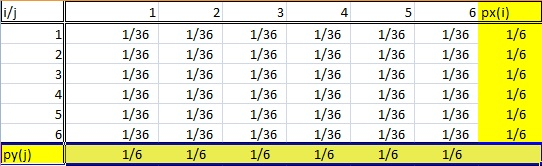
\includegraphics[width = .8\textwidth]{figure/marginal-distributions-1.jpg}
	\caption{用过Excel的同学都知道什么是边缘分布律}
\end{figure}

\noindent
\textbf{独立性等价于可以分解为相乘!}
\begin{itemize}
	\item 事件$A$与$B$独立 \;$\Longleftrightarrow$\; $P(AB) = P(A) P(B)$; 
	\item 随机变量$X$与$Y$独立 \;$\Longleftrightarrow$\; $F(x,y) = F_X(x)F_Y(y)$; 
	\item 离散型$X$与$Y$独立 \;$\Longleftrightarrow$\; $P\{X = x_i, Y = y_j\} = P\{X = x_j\} P\{Y = y_j\}$; 
	\item 连续型$X$与$Y$独立 \;$\Longleftrightarrow$\; $f(x, y) = f_X(x) f_Y(y)$. 
\end{itemize}
\begin{corollary}
	若随机变量$X$与$Y$独立, 则$E(XY) = E(X) E(Y)$.
\end{corollary}
\begin{corollary}
	若随机变量$X$与$Y$独立, 则它们的连续函数$g(X)$与$h(Y)$也独立. 
\end{corollary}

对于离散分布, 我们还要求掌握\textbf{条件分布律}. 
若$P\{Y_j > 0\}$, 则称
$$
P\{X=x_i|Y=y_j\}=\frac{P\{X=x_i,\:Y=y_j\}}{P\{Y=y_j\}},\quad i=1,2,\cdots 
$$
为在$Y=y_j$的条件下随机变量$X$的条件分布律; 同样的, 若$P\{X_i > 0\}$, 则称
$$
P\{Y=y_i|X=x_i\}=\frac{P\{X=x_i,\:Y=y_j\}}{P\{X=x_i\}},\quad j=1,2,\cdots 
$$
为在$X=x_i$的条件下随机变量$Y$的条件分布律. 

二维有界区域$G$上的\textbf{均匀分布}的密度函数为
\begin{equation*}
	f(x, y) = 
		\begin{cases}
			\frac{1}{|G|}, &(x, y) \in G \\ 0, & \text{其它}. 
		\end{cases}
\end{equation*}
\textbf{二维正态分布}$(X,Y) \sim N(\mu_1, \mu_2, \sigma_1^2, \sigma_2^2, \rho)$由五个参数控制, 其中边缘分布$X \sim N(\mu_1, \sigma_1^2)$, $Y \sim N(\mu_2, \sigma_2^2)$, 参数$\rho \in [ -1, 1]$则是$X$和$Y$的相关系数. 

 \noindent\textbf{随机变量函数的分布.}
设随机变量$(X,Y)$的联合分布函数为$F(x,y)$. 
 
\textbf{最大值}$Z = \max\{X, Y\}$的分布函数为
\begin{equation*}
	F_Z(z) 
	= P\{\max\{X, Y\} \leq z\}
	= P\{X \leq z, Y \leq z\}
	= F(z,z). 
\end{equation*}
特别当$X$和$Y$独立时$F_Z(z) = F_X(z) F_Y(z)$. 
\textbf{最小值}$Z = \min\{X,Y\}$的分布函数为
\begin{align*}
	F_Z(z)
	&= 1 - P\{\min\{X, Y\} > z\}
	= 1 - P\{X > z, Y > z\} \\
	&= 1 - \left[ 1 - F_X(z) - F_Y(z) + F(z,z) \right].
\end{align*}
特别当$X$和$Y$独立时$F_Z(z) = 1 - [1- F_X(z)][1- F_Y(z)]$. 

离散型随机变量之和的分布律有离散卷积公式
$$
\begin{aligned}
	P\{X+Y=z_k\}
	&=\quad\sum_iP\{X=x_i,\:Y=z_k-x_i\}\\
	&=\quad\sum_jP\{X=z_k-y_j,\:Y=y_j\},\quad k=1,2,\cdots
\end{aligned}
$$
连续型随机变量之和有卷积公式
$$
\begin{aligned}
	f_{X+Y}(z)
	=\int_{-\infty}^{+\infty}f(x,z-x)\dd x
	=\int_{-\infty}^{+\infty}f(z-y,y)\dd y.
\end{aligned}
$$

\subsection{例题示范}

\begin{example}
	从$(0,1)$中随机地取两个数,求积不小于$3/16$、和不大于$1$的概率.
\end{example}
\begin{solution}
	设取出的两个数分别为$X$和Y,则$(X,Y)$的联合密度函数为
	\begin{equation*}
		f(x, y) = 
			\begin{cases}
				1, & 0 < x < 1, 0 < y < 1, \\
				0, & \text{其它}. 
			\end{cases}
	\end{equation*}
	于是
	\begin{align*}
		P\{XY \geq 3/16, X + Y \leq 1\}
		&= \int_{1/4}^{3/4} \int_{3/16x}^{1-x} \dd y \dd x
		= \int_{1/4}^{3/4} \left( 1 - x - \frac{3}{16 x} \right) \dd y \dd x \\
		&= \left(x - \frac{x^2}{2} - \frac{3}{16} \ln x \right)_{1/4}^{3/4}
		= \frac{1}{4} - \frac{3}{16} \ln 3. 
	\end{align*}
\end{solution}

\begin{example}
设二维随机变量$(X,Y)$的联合密度函数如下,试问$X$与$Y$是否相互独立?
$$
	f(x,y)=
	\begin{cases}
		x e^{-(x+y)}&\:x\:>\:0\:,y\:>\:0\:,\\\:0\:,&\:\text{其它}
	\end{cases}
$$
\end{example}
\begin{solution}
	当$x>0$时, 边缘密度$f_X(x) = \int_0^{\infty} x e^{-(x+y)} \dd y = x e^{-x}$. 
	当$y>0$时, 边缘密度$f_Y(y) = \int_0^{\infty} x e^{-(x+y)} \dd x = e^{-y}$. 
	于是由$f_X(x) f_Y(y) = f(x,y)$知$X$与$Y$相互独立. 
\end{solution}

\begin{example}
$(X,Y)$的联合密度函数为
$$
f(x,y)=\begin{cases}3x,&0<x<1,\quad0<y<x,\\0,&\text{其他}.\end{cases}
$$
求$Z = X - Y$的密度函数. 
\end{example}
\begin{solution}
	$\{x - y \leq z\} = \{y \geq z - z\}$在$z \in (0,1)$时与$f(x,y)$的非零区域有交集. 
	于是当$z \in (0,1)$时, 
	\begin{align*}
		F_Z(z) 
		& = P\{X - Y \leq z\}
		= \int_0^z \int_0^x 3 xy \dd y \dd x + \int_z^1 \int_{x-z}^x 3 xy \dd y \dd x \\
		& = \frac{3z}{2} - \frac{z^3}{2}, 
	\end{align*}
	从而$Z$的密度为
	\begin{equation*}
		f_Z(z) = 
		\begin{cases}
			\frac{3}{2}(1 - z^2), &0 < z < 1, \\
			0, &\text{其它}. 
		\end{cases}
	\end{equation*}
\end{solution}


























\end{document}